\chapter{Coupling Dynamics to Physics in ICONAM}

\section{The Coupling Interface}
The motivation to create a coupling interface between physics and dynamics comes from several demands
\begin{enumerate}
\item have a clean port to dock the physical parametrizations when new developments come into the model

\item define all fields and variables coming from the dynamics at one place to be valid for all schemes

\item to recalculate the prognostic fields from the dynamical core in different definition (e.g. $\theta_v$) or from different place (winds at the edges and not at the center) forth and back.

\end{enumerate}

\subsection{Flow of Physic Calls}

One important task of the interface is the organisation of physical contributions to the prognostic variables.

In order to be stable and consistent but also efficient in computation we do a compromise between sequential and accumulated updating of the prognostic stage of our fields. Therefore we consider some physical processes as fast ones which should update their contributions in a cumulative way, meaning that each process see the contributions of the one acting before it. Currently the cloud microphysics, the turbulence scheme and the surface model fall into this category.\\

At which place the surface model has to be called is still under discussion.

Other processes are considered to act more slowly on the atmosphere. Therefore they will be called less often, they see the updated stage of the fast processes and  they give out \emph{tendencies} working on the dynamical fields at the next time step. These are the radiation, convection, cloud cover, and the gravity wave related schemes.\\

This introduces an additional complexity and care must be taken on the place and time of the diagnostic of the variables \emph{temperature} and \emph{pressure}
The overall flow - how physics works together with dynamics is scetched in Figure{\ref{flux}}. The full inner flow is described below:

\begin{itemize}

\item THE FAST PROCESSES
\begin{enumerate}

\item \texttt{CALL nh\_update\_prog\_phy} The hydrometeor variables are updated at first, immediately after their advection is completed.
\item \texttt{CALL diagnose\_pres\_temp} Temperature and pressure will be diagnosed  out of exner pressure and the moist potential temperautre on both half and full levels.

\item \texttt{CALL satad\_v\_3D} The saturation stage of the atmosphere is checked and water vapor is converted into cloud water or vice versa.

\item Out this the set of prognostic fields is recalculated and so updated.

\item \texttt{CALL rbf\_vec\_interpol\_cell } Interpolation of winds from egdes to cells

\item \texttt{CALL diagnose\_pres\_temp }diagnose Pressure, Temperature at half and full levels

\item  \texttt{CALL nwp\_turbulence} Currently the COSMO turbulence and the ECHAM turbulence scheme are available
\item \texttt{CALL diagnose\_pres\_temp} only diagnose pressure, since temperature is at actual state!
\item  \texttt{CALL nwp\_microphysics} Currently this leads to the current COSMO microphysics with 5 prognostic hydrometeors.

\item \texttt{CALL pre\_radiation\_nwp} calculates the zenith angle for the heating rates
\item \texttt{CALL radheat} heating rates are calculated each time step
\item recalculate the prognostic variables

\end{enumerate}


\item  THE SLOW PROCESSES
\begin{enumerate}
\item \texttt{CALL diagnose\_pres\_temp }
At the first timestep diagnose Pressure and temperature, later on only the pressure needs to be diagnosed since temperature is up to date.
\item \texttt{CALL nwp\_convection} Currently the Tiedtke-Bechtold code is implemented
\item \texttt{CALL cover\_koeh} 3 different types of cloud diagnostics are behind.
\item \texttt{CALL nwp\_radiation} two Radiation sets: RRTM and Ritter-Geleyn
\item \texttt{CALL pre\_radiation\_nwp} calculates the zenith angle for the heating rates
\item \texttt{CALL radheat} heating rates are calculated each time step because of the diurnal cycle
\item \texttt{CALL nwp\_sso}
\item \texttt{CALL nwp\_gwd}

\item collect the scalar tendencies of the slow processes

\item recalculate the prognostic variable

 convert temperature tendencies into exner tendencies
 Since the exner function shows up as $\Pi=\frac{T_v}{\theta_v}$ this relates
 to pressure and virtual temperature tendencies

\bea
 \frac{d \pi}{d t} = \frac{1}{c_{pd} \theta_v \rho} \, \frac{dp}{d t} \\
 \frac{dp}{d t} = (c_p/c_v -1) Q_h + c_p/c_v Q_h\\
  \mbox{ where}\;  Q_h = \frac{d T}{d t} |_{phys} \\
  \mbox{ and}\; Q_m = R_d \,T \,\rho \frac{d \alpha}{d t} .
\eea

The resulting tendency can be written as
\be
 \frac{d \pi}{d t}= \frac{R}{c_{v} \theta_v} \left( \frac{d T}{dt} \\
                        + T \frac{d \alpha}{ d t} \right) 
\ee

\end{enumerate}


\end{itemize}

\begin{figure}
\begin{center}
\rotatebox{90}{\scalebox{0.8}{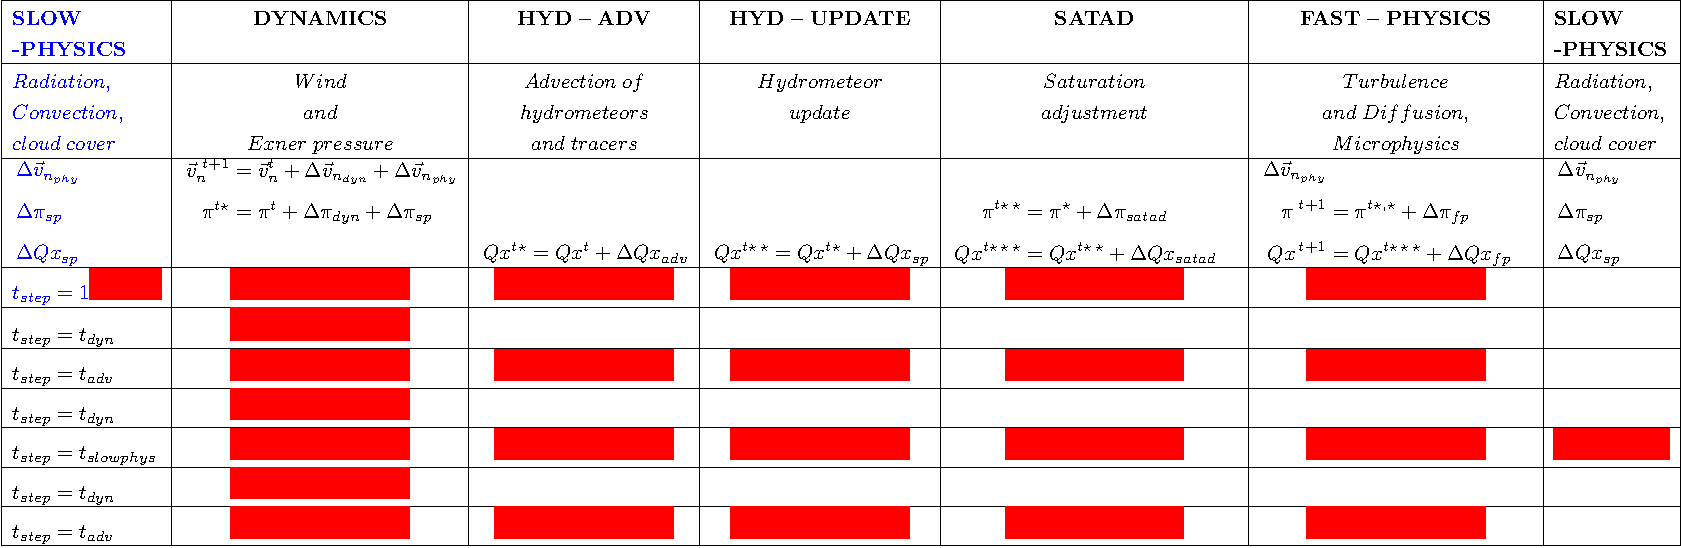
\includegraphics{flux_diagram-crop.pdf}}}
\end{center}
\caption{Application flow of Physics calls}
\label{flux}
\end{figure}
